\documentclass[8pt,a4paper,twocolumn]{article}

%%%%%%%%%%%%%%%%%%%%%%%%%%%%%%%%%%%%%%%%%%%%%%%%%%%%%%%%%%%%%%%%%%%%%%%%%%%%%%%%%%%%%%%% - Package Begin
%% Margins
\usepackage[left=2cm, right=2cm, top=2cm, bottom=2cm]{geometry}

%% Type & Text
\usepackage[utf8]{inputenc}
\renewcommand*\rmdefault{ppl}
\usepackage{csquotes}

%% Math & Equations
% American Mathematical Society (AMS) plain Tex macros
% The amsmath package is the principal package in the AMS-LaTeX distribution
% The amsfonts package provides extended TeX fonts
% The amssymb package provides various useful mathematical symbols
% The amsthm package provides extended theorem environments
\usepackage{amsmath}
\DeclareMathSizes{7}{7}{3}{3}
\usepackage{pifont}
\usepackage{amsfonts}
\usepackage{amssymb}
\usepackage{mathrsfs}
\DeclareMathOperator*{\argmin}{arg\,min}
\DeclareMathOperator*{\argmax}{arg\,max}
\usepackage{dcolumn}% Align table columns on decimal point
\usepackage{bm}% bold math
\usepackage{algorithm}
\usepackage{algpseudocode}
\algnewcommand\textproc{\textsc}
\usepackage{upgreek}

% New command to refer to equations as Eq.(1),Eq.(2),...
\newcommand{\eqnref}[1]{Eq.(\ref{#1})}

%% Color
\usepackage[x11names]{xcolor}
\usepackage{tcolorbox}

%% Define main accent color
\definecolor{main.green}{rgb}{0.0, 0.27, 0.13}

%% Define support accent colors
\definecolor{support.grey}{rgb}{0.33, 0.33, 0.33} % Dark grey

%% Sections
% Section numbers with trailing dots.
\usepackage{secdot}
\usepackage{epstopdf}

%% Also put a dot after the subsection number
\sectiondot{subsection}

%% Set a space between dot and heading text
\sectionpunct{section}{. } % By default, \sectiondot places a \quad
\sectionpunct{subsection}{. } % after the number
\usepackage{titlesec}
\titleformat{\section}
    {\sffamily\bfseries\color{main.green}}{\thesection\quad}{\rule[-0.35cm]{1.5pt}{1cm}\quad}{\MakeUppercase}

%% Subsections
\titleformat{\subsection}
%   {\normalfont\bfseries\itshape\color{main.green}}{\thesubsection}{1em}{}
  {\sffamily\bfseries\itshape\color{main.green}}{\thesubsection}{1em}{}

%% Subsubsections
\titleformat{\subsubsection}
  {\sffamily\itshape\color{main.green}}{\thesubsubsection}{1em}{}

%% Figures & Graphics
\usepackage{subcaption}
\usepackage[justification=left]{caption}
\usepackage[skip=2pt,font=scriptsize]{caption}
\renewcommand{\figurename}{\textbf{Fig.}}
\usepackage[labelsep=endash]{caption}
\usepackage{graphicx}
\usepackage{siunitx}
\usepackage{float}

%% List
\usepackage{listings}
\usepackage{enumitem}

%% Tables
\usepackage{pgfplotstable}
% global settings
\pgfplotstableset{
    every head row/.style={
    before row=\toprule,after row=\midrule},
    every last row/.style={
    after row=\bottomrule},
    col sep = &,
    row sep=\\,
    string type,
}

%% Title
\makeatletter
\renewcommand{\maketitle}{\bgroup\setlength{\parindent}{0pt}
\vspace{2.5cm}
\begin{flushleft}
  \textbf{\@title}

  \@author
\end{flushleft}\egroup
}
\makeatother

%% Abstract
\renewcommand\abstractname{\normalfont\textsc{
    \begin{flushleft}
        \textbf{\textcolor{support.grey}{ABSTRACT}}
    \end{flushleft}
    }
    \vspace{-4mm}
}

%% Footnotes
\usepackage[hang,flushmargin]{footmisc}

%% digitalepidemiology -- Header
\usepackage{fancyhdr}
\pagestyle{fancy}
\lhead{\normalfont\textcolor{main.green}{\textbf{Digital Epidemiology:}} \textcolor{support.grey}{\textit{Sentiment Analysis Architectures, Algorithms, \& Applications for Disease Ecology}}}
\rhead{\textcolor{main.green}{\textbf{\thepage}}}
%%%%%%%%%%%%%%%%%%%%%%%%%%%%%%%%%%%%%%%%%%%%%%%%%%%%%%%%%%%%%%%%%%%%%%%%%%%%%%%%%%%%%%%% - Package End

%%%%%%%%%%%%%%%%%%%%%%%%%%%%%%%%%%%%%%%%%%%%%%%%%%%%%%%%%%%%%%%%%%%%%%%%%%%%%%%%%%%%%%%% - Title Begin

% digitalepidemiology -- Title
\title{\normalfont\huge{\textcolor{main.green}{\textbf{Digital Epidemiology:}}}\\
\textit{Sentiment Analysis Architectures, Algorithms, \\ \& Applications for Disease Ecology}\vspace{1.0cm}}

% digitalepidemiology -- Author Information
\author{
    \normalsize{Erick Oduniyi (\textbf{eeoduniyi@gmail.com})}\\
    \textit{This document was prepared for the members of the University Of Kansas' Agusto Epidemiology Lab}
}

% Suppress date information
\date{}

% Supress page numbering at the bottom
\fancyfoot[C]{}
%%%%%%%%%%%%%%%%%%%%%%%%%%%%%%%%%%%%%%%%%%%%%%%%%%%%%%%%%%%%%%%%%%%%%%%%%%%%%%%%%%%%%%%% - Title End

%%%%%%%%%%%%%%%%%%%%%%%%%%%%%%%%%%%%%%%%%%%%%%%%%%%%%%%%%%%%%%%%%%%%%%%%%%%%%%%%%%%%%%%% - Document Begin
\begin{document}

% digitalepidemiology -- Abstract
\twocolumn[
\begin{@twocolumnfalse}
\maketitle
	\vspace{-.25cm}
\frenchspacing
\begin{abstract}
\noindent The goal of this document is to review the standard sentiment analysis methods and their associated advantages and disadvantages. In the end, this will provide a platform to sensibly implement sentiment analysis algorithms reliably for any domain and application of interest. In route and in particular, we review and provide basic examples of these algorithms along the way, and finally outline how they could be used in epidemiology and assessing the public's health through data mining platforms.
\end{abstract}
\vspace{1.0cm}
\end{@twocolumnfalse}
]

% digitalepidemiology -- Introduction
\section{Introduction}
\frenchspacing
The ability to understand or infer emotion signatures from an individual's information: text, speech, pictures, art works has always generated healthy amounts of engineering and scientific interest. Now, in the current information age where social-media platforms like Facebook, Instagram, and Twitter attract and interconnect individuals from around the world, understanding these emotion characteristics have become critical. Indeed, these social media platforms offer individuals the ability to express and disseminate their self expression; instantaneously highlighting their personalities to the world. Hence, social media platforms offer potentially rich digital representations of humanity at large. Because of the large amounts personality representations, anthropologist, psychologist, and sociologist might be able to glean a unique understanding of human nature through automated belief and opinion mining and subsequent analysis. Principally, this automated emotion analysis is possible because of \textit{sentiment analysis}. As a result, it has become increasingly common practice to unleash sentiment analysis methods for the prediction of election outcomes, commerce and marketing, user satisfaction, and general behavioral analysis online.


% digitalepidemiology -- Sentiment Analysis
\thispagestyle{empty}
\section{Sentiment Analysis}
\frenchspacing
\textit{Sentiment analysis} refers to the automated process of extracting the underlying affect in content. More, sentiment analysis makes use of tools from the field of natural language processing and computational linguistics to study polarity, affect, and subjective information (e.g., speech, text, images). Assessing the \textit{polarity} -- the degree to which a text is \textit{positive}, \textit{negative}, or \textit{neutral} is often the most basic task\footnote{The assumption of virtually all sentiment analysis algorithms is that people have a general understanding of things that are \textit{very positive} and \textit{very negative}} of sentiment analysis. 
While extracting \enquote{sentiment} -- \textit{affective states} $\in$  $\lbrace$\enquote{angry}, \enquote{sad}, \enquote{happy}, $... \ \rbrace$ is a slightly more sophisticated sentiment analysis endeavor.

To avoid misunderstanding, it is necessary to specify that \textit{emotion} and sentiment are not equivalent. Emotion is typically believed to be instinctive, triggered by psychological responses to direct experiences. We often try and capture emotion with cultural concepts like happiness, sadness, fear, and surprise. While sentiment is certainly influenced by emotion, sentiment describes the mental attitudes individuals have towards things (i.e., opinion) which is formed by cultural meaning. Thus, when talking about sentiment analysis, individuals introduce the concept of polarity to tie together emotion and sentiment, where content can have a positive (or slightly positive or very positive), neutral, and negative (or slightly negative or very negative). Despite this and other sentiment analysis conventions, there are a few general difficulties of the sentiment analysis practice. Here, they are outlined as such:

\begin{itemize}
\item \textit{Extremely difficult to develop a general sentiment analysis tool. It is always necessary to train and identify domain specific sentiment. }
\item \textit{Complex sentences that contain sarcasm, irony, context, negation, qualifiers, and multiple subject attitudes are difficult to account for. In fact, many sentiment analysis tools do not account for such complexity.}
\item \textit{Human judgment is used to asses the accuracy of sentiment analysis tools. However, it is impossible to get human raters to unanimously agree on sentiment. Thus, the ballpark for accuracy is limited.}
\end{itemize}

Despite these general complications, sentiment analysis still offers the ability for one to break down human generated text and information into  sequences of emotions, so that the relationship between emotional content and other variables might be explored.

\subsection{Sentiment Analysis Methods}
Typically sentiment analysis is done by utilizing machine learning methods or dictionary-based look up algorithms. Machine learning methods require rich domain specific data, and could take longer to implement due to training, but also return more accurate results. For text, dictionary-based methods allow users to access the polarity of specific words, which provides a granular look at the perceived emotional content. Both methods must make use of human analysis, where individual ratings of content are aggregated. 

\subsubsection{Dictionary-based}
\textit{Dictionary-based} or \textit{lexicon-based} sentiment analysis methods use a \textit{sentiment dictionary} or \textit{sentiment lexicon}, where words are annotated by a \textit{polarity score}. 
Then, the specified \textit{dictionary-based sentiment analysis algorithm} takes in the content word-by-word assessing the individual word polarities and then finally producing some average or aggregated score of the entire content.

\paragraph{Dictionary look-up algorithms}
In general, the \textit{dictionary-based sentiment analysis procedure} can be described as:

\begin{enumerate}
\item \textbf{Tokenization }-- For each paragraph $p_i$, we break into a set of sentences $p_i = \lbrace s_1, s_2, \ ... \ , s_3 \rbrace$ Then, for each sentence $s_i$, we break into a set of words $s_i = \lbrace w_1, w_2, \ ... \ , w_n \rbrace$. 
\item \textbf{Rating} -- We'll denote $w_{i,j,k}$ as the $k^{th}$ word in the $j^{th}$ sentences of the $i^{th}$ paragraph. For each word $w_{i,j,k}$, search through the respective sentiment dictionary. Give words that are positive a score of +1 and words that are negative a score of -1.
\item \textbf{Aggregation} -- Depending on the sophistication of the dictionary algorithm, for each sentence we perform a count of the positive and negative words, take the \textit{absolute proportional difference}, or \textit{relative proportional difference}:
\end{enumerate}

\begin{align}
Sentence \ Polarity = w_+ - w_-
\end{align}
\begin{align}
Sentence \ Polarity = \dfrac{w_+ - w_-}{w_+ + w_- + w_0}
\end{align}
\begin{align}
Sentence \ Polarity = \dfrac{w_+ - w_-}{w_+ + w_-}
\end{align}
Where $w_-, w_+, w_0$ denote the total positive, negative, and neutral words in a sentence, respectively.

\subsubsection{Dictionaries}
Syuzhet uses three standard sentiment dictionaries: \textit{nrc, afinn, bing}, and a custom sentiment dictionary \textit{syuzhet}. Syuzhet augments its sentiment analysis based on each dictionary. Sentimentr makes use of the same dictionaries as syuzhet and pattern.nlp is composed of its own list of adjectives.

A variety of lexicon-based sentiment analysis algorithms and their sentiment dictionaries can be found in many packages and libraries within the programming languages Python and R. For example, Python's \textit{pattern.nlp} and \textit{natural language toolkit} (NLTK) offer some of the most comprehensive library of natural language processing tools, of which include dictionary and classification-based sentiment analysis methods. More, with Python's highly popular \textit{sckit-learn} package, students and researchers can utilize a variety of machine learning methods in combination with NLTK to generate robust sentiment extraction tools. Likewise, R has a number of dictionary-based sentiment analysis tools available in the following R libraries: \textit{syuzhet}, \textit{sentimentr}, \textit{tm}. 

For both Python and R, each of these lexicon-based algorithms utilize a different analysis and aggregation schema (e.g., absolute proportional difference or relative proportional difference). Even more, while the pattern.nlp package was originally developed for python, it is possible to cross-compile its functions for R. Pattern.nlp is composed of a list of adjectives in English, French, Dutch, and Spanish that occur frequently in product reviews. Worth noting, unlike the other dictionary-based sentiment analysis algorithms, pattern.nlp performs sentiment analysis by taking the \textbf{average of the adjectives within a sentence} opposed to the absolute or proportional difference of \textbf{all} words. 

As an example of this difference, we will examine the following sentence with pattern.nlp and compare the results to other dictionary-based algorithms:

\begin{center}{\textit{"The movie attempts to be surreal by incorporating various time  paradoxes, but it's presented in such a ridiculous way it's seriously boring."}}\end{center}

\begin{table}[H]
\begin{center}
\pgfplotstabletypeset{
Algorithm    & pattern  & nrc  & afinn  & syuzhet  \\ 
Pattern.nlp & x & -- & -- & -- \\ 
SentimentR & -- & x & x & x \\
Syuzhet  & -- & x & x & x \\
}
\vspace{1.5mm}
\caption{Comparing performance on \enquote{The movie...} between pattern.nlp to sentimentr and syuzhet: nrc, afinn, bing, syuzhet}
\end{center}
\end{table}
\begin{table}[H]
\begin{center}
\pgfplotstabletypeset{
Human   & Rating  & Subjectivity \\ 
1 & -- & -- \\ 
2 & -- & -- \\
3 & -- & -- \\
}
\vspace{1.5mm}
\caption{Comparing performance on \enquote{The movie...} between human participants}
\end{center}
\end{table}

Pattern.nlp returns a sentiment score of $-0.34$ as it is the average sentiment score of \textit{surreal}, \textit{various}, \textit{ridiculous} and \textit{seriously boring}. Syuzhet makes use of relative proportional difference and four different sentiment dictionaries. Sentimentr is an augmentation of syuzhet, where it tries to account for \textit{valence shifters} (negators, amplifiers, de-amplifiers, and adversative conjunctions)

% Figure: Classification-based sentiment analysis
\begin{figure}
\centering
\begin{subfigure}[b]{.50\textwidth}
   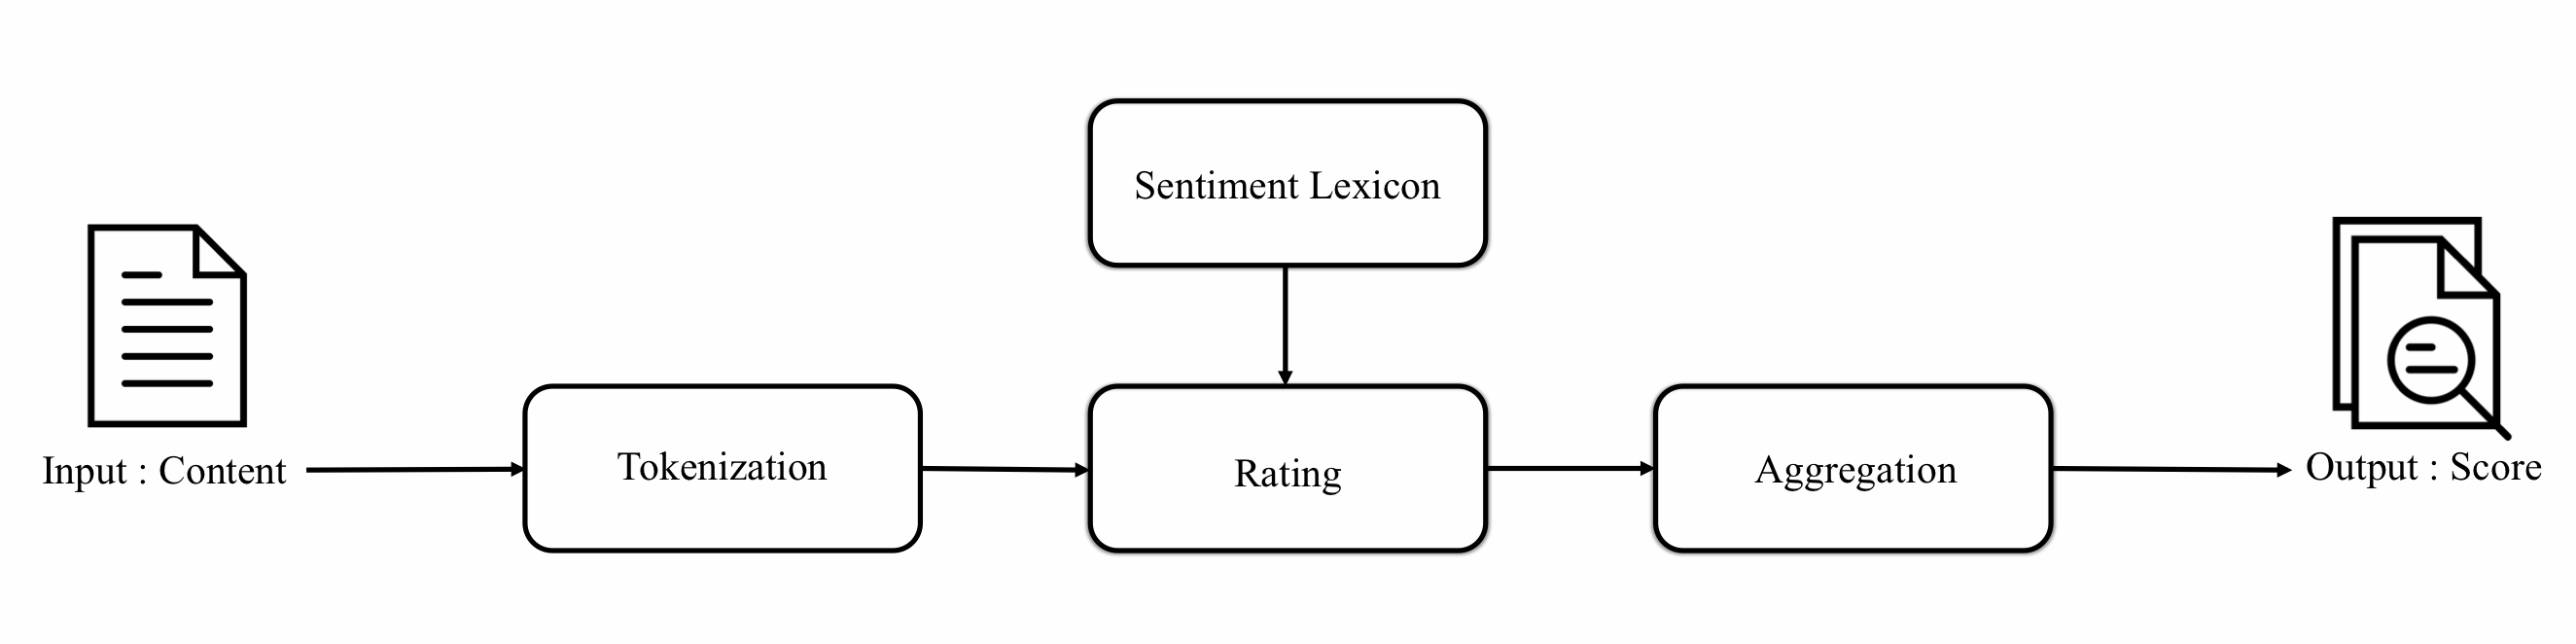
\includegraphics[width=1\linewidth]{img/lexicon-arch-1.png}
   \caption{}
   \label{fig:Ng1} 
\end{subfigure}

\begin{subfigure}[b]{.50\textwidth}
   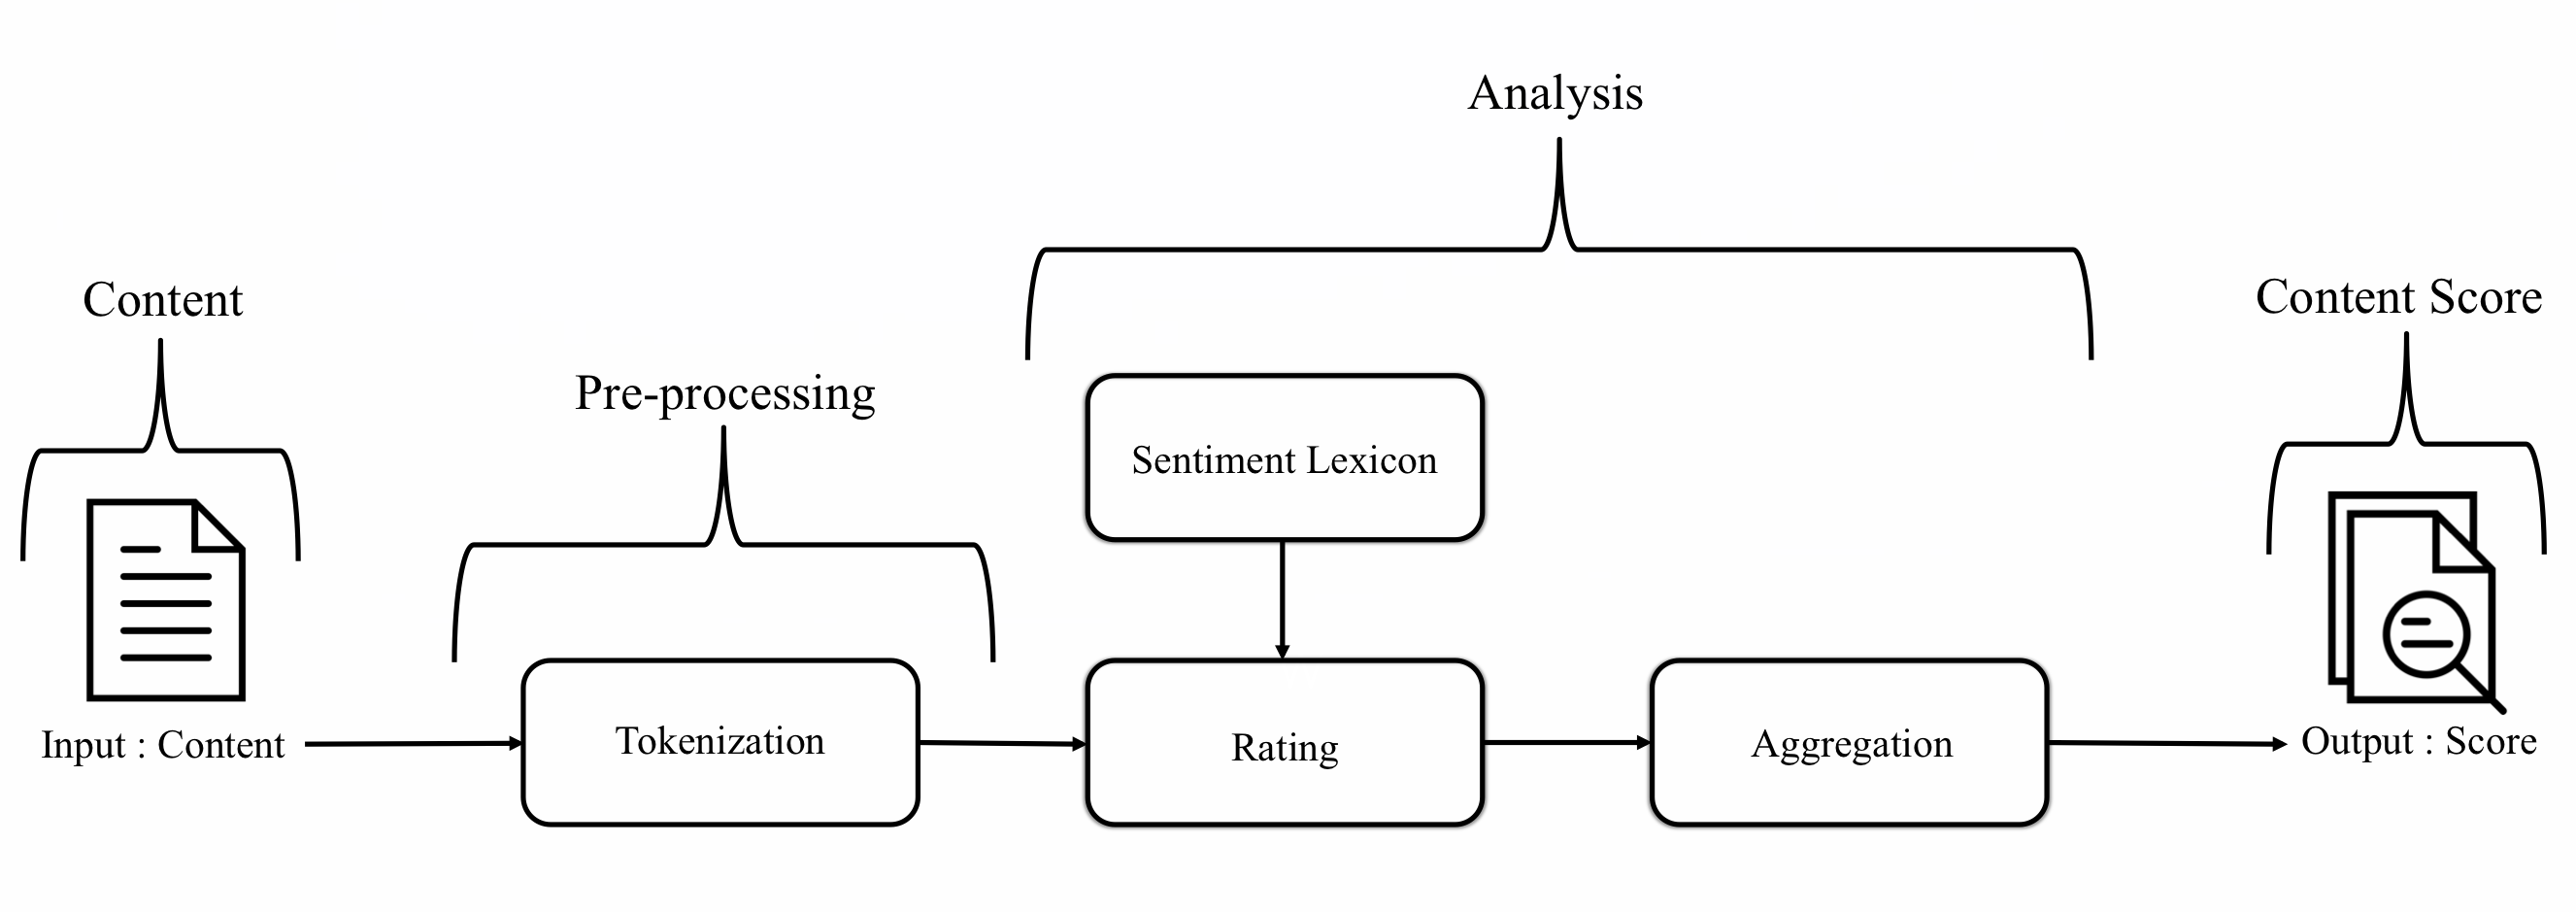
\includegraphics[width=1\linewidth]{img/lexicon-arch-2.png}
   \caption{}
   \label{fig:Ng2}
\end{subfigure}

\caption[sentimentanalysisarchitecture]{Typical systems architecture of lexicon-based sentiment analysis, where \textbf{(a)} and \textbf{(b)} show the non-annotated and annotated system process respectively.}
\end{figure}

\begin{algorithm}[H]
\caption{\textit{Word-Tokenization}}
\label{array-sum}
\begin{algorithmic}[1]
\State \textbf{let} $Content = $ {\scriptsize{$\lbrace paragraph_1, paragraph_2, \ ... \ , paragraph_n \rbrace$}} 
\Function{Tokenizer}{$Content$}
\State \textbf{let} $\tilde{W} = \lbrace \rbrace$
\For{$paragraph_i$ = $1:n$}
% \For{$paragraph$ in $Content$}
    \State \textbf{let} $paragraph_i = $ {\scriptsize{$\lbrace sentence_1, sentence_2, \ ...\ , sentence_m \rbrace$}}
    \For{$sentence_j$ = $1:m$}
        \State \textbf{let} $sentence_j = \lbrace w_{i,j,1}, w_{i,j,2}, \ ...\ , w_{i,j,k} \rbrace$
        \State $\tilde{W} = \lbrace \tilde{W}, sentence_j \rbrace$
    \EndFor
\EndFor \\
\Return $\tilde{W}$
\EndFunction
\end{algorithmic}
\end{algorithm}

% Algo: Dictionary-based sentiment analysis
\begin{algorithm}[H]
\caption{\textit{Dictionary-based}}
\label{array-sum}
\begin{algorithmic}[1]
\Procedure{sentimentAnalysis}{$Content, Dict$}
\State $\tilde{W} = $  \textproc{Tokenizer}($Content$)
\Function{Rater}{$\tilde{W}$}
    \State \textbf{let} $w^+ = \lbrace \rbrace$; \ $w^- = \lbrace \rbrace$; \ $w^0 = \lbrace \rbrace$
\For{$w_{i,j,k}=1: |\tilde{W}|$} 
    \If{$w_{i,j,k} \in Dict^+$}
       \State $w^+ = \lbrace w^+,w_{i,j,k}\rbrace$
    \ElsIf{$w_{i,j,k} \in Dict^-$}
        \State $w^- = \lbrace w^-,w_{i,j,k}\rbrace$
    \Else  
        \State $w^0 = \lbrace w^0,w_{i,j,k}\rbrace$
    \EndIf
\EndFor
    \State $\tilde{W}_{rated} = (w^+,w^-,w^0)$
\EndFunction
\Function{Aggregate}{$\tilde{W}_{rated}$}
\State $Content_{score} = {\scriptsize{\dfrac{w_+ - w_-}{w_+ + w_- + w_0}}}$
\EndFunction \\
\Return ${Content_{score}}$
\EndProcedure
\end{algorithmic}
\end{algorithm}

\subsubsection{Main Advantages}
The strongest asset of this technique is that it does not require any training data.

\subsubsection{Main Disadvantages}
Dictionary-based approaches weakest points are the requirement of a large enough number of words and their associated polarity scores or annotations. Additionally, sentences, and larger-level language expressions are not included in sentiment lexicons. 

\subsubsection{Machine-learning-based}
The sentiment analysis task is usually modeled as a classification problem where a classifier is fed with a text and returns the corresponding category, e.g. positive, negative, or neutral (in case polarity analysis is being performed).

\subsubsection{Feature extraction}
To perform ML-based sentiment analysis, one first must represent the sentences in some vector space. Frequency-based methods are commonly used to represent a sentence either by a bag-of-words, which is a list of the words that appear in the sentence with their frequencies, or by a term frequency-inverse document frequency (tf-idf) vector where the word frequencies in our sentences are weighted with their frequencies in the entire corpus.

\begin{algorithm}[H]
\caption{\textit{Feature Extraction}}
\label{array-sum}
\begin{algorithmic}[1]
\Procedure{featureExtraction}{}
\EndProcedure
\end{algorithmic}
\end{algorithm}
\subsubsection{Naive Bayes}
A family of probabilistic algorithms that uses Bayes's Theorem to predict the category of a text.

\subsubsection{Linear Regression}
The most basic algorithm in statistics for the prediction of the dependent variable $Y$ given a set of features or dependent vairable $X$.

\subsubsection{Support Vector Machines}
A non-probabilistic model which uses a representation of text examples as points in a multidimensional space. These examples are mapped so that the examples of the different categories (sentiments) belong to distinct regions of that space.. Then, new texts are mapped onto that same space and predicted to belong to a category based on which region they fall into.

\subsubsection{Deep Learning}
% A diverse set of algorithms that attempts to imitate how the human brain works by employing artificial neural networks to process data.

% To build a deep-learning model for sentiment analysis, we first have to represent our sentences in a vector space. We studied frequency-based methods in a previous post. They represent a sentence either by a bag-of-words, which is a list of the words that appear in the sentence with their frequencies, or by a term \textit{frequency-inverse document frequency} (tf-idf) vector where the word frequencies in our sentences are weighted with their frequencies in the entire corpus.

% These methods are very useful for long texts. For example, we can describe very precisely a newspaper article or a book by its most frequent words. However, for very short sentences, it's not accurate at all. First, because 10 words are not enough to aggregate. But also because the structure of the sentence is very important to analyze sentiment and tf-idf models hardly capture negations, amplifications, and concessions. For instance, \enquote{Very good food, but bad for service... would have the same representation} as \enquote{Bad for food, but very good service!}

% Figure: Classification-based sentiment analysis
\begin{figure}[h]
 \centering
 \includegraphics[width=0.90\textwidth]{}
 \caption{Typical systems architecture of classification-based sentiment analysis.}
 \label{fig:dictionary-based-framekwork}
\end{figure}

% Algo: Classification-based sentiment analysis
\begin{algorithm}[H]
\caption{\textit{Machine-Learning-based}}
\label{array-sum}
\begin{algorithmic}[1]
\Procedure{sentiClassification}{}
\EndProcedure
\end{algorithmic}
\end{algorithm}
\subsubsection{Main Advantages}
\subsubsection{Main Disadvantages}
\subsection{Combined Approach -- Hybrid Systems}
The combination of machine learning and lexicon-based approaches to address sentiment analysis is called Hybrid. Though not commonly used, this method usually produces more promising results than the approaches mentioned above.

% Figure: Hybrid-based sentiment analysis
\begin{figure}[h]
 \centering
 \includegraphics[width=0.90\textwidth]{}
 \caption{Typical systems architecture of hybrid-based sentiment analysis.}
 \label{fig:dictionary-based-framekwork}
\end{figure}

% Algo: Hybrid-based sentiment analysis
\begin{algorithm}[H]
\caption{\textit{Hybrid}}
\label{array-sum}
\begin{algorithmic}[1]
\Procedure{sentimentHybrid}{}
\EndProcedure
\end{algorithmic}
\end{algorithm}
\subsubsection{Main Advantages}
\subsubsection{Main Disadvantages}
\subsection{Evaluating Sentiment Analysis Methods}
\section{Emotion Recognition Systems}
\section{Applying Sentiment Analysis}


% digitalepidemiology -- Conclusion
% \input{06_conclusion.tex}

% digitalepidemiology -- References
\bibliographystyle{unsrt}
\bibliography{references}
%%%%%%%%%%%%%%%%%%%%%%%%%%%%%%%%%%%%%%%%%%%%%%%%%%%%%%%%%%%%%%%%%%%%%%%%%%%%%%%%%%%%%%%% - Document End
\end{document}
